\documentclass[working]{article}

\input{preamble}
% Warning: this template does not support Chinese.

\geometry{a4paper,left=2cm,right=6cm,top=2cm,bottom=2cm}
\setlength{\marginparwidth}{4cm}
\linenumbers
\bibliographystyle{abbrvnat}
% \setcitestyle{numbers,open={[},close={]},comma,super}
\setcitestyle{authoryear,open={(},close={)},comma}

\title{Mathematical Notes}
\author{Foo Bar}
\date{\today}

\begin{document}

\maketitle

% \begin{framed}{\large
% TODO list of the following week
% \begin{itemize}
%     \item Finish the note organization work of Part II
%     \item Read Chapters 9 and 10
%     \item Course works
% \end{itemize}
% }
% \end{framed}

This is a test.

An introduction to the note draft template\cite{pml1Book},\cite{pml2Book}.

\section{Figures}
\begin{figure}[htbp]
    \centering
    \begin{tikzpicture}[scale=0.8]
        % Define node styles
        \tikzstyle{block} = [rectangle, draw, fill=blue!20, 
            text width=5em, text centered, rounded corners, minimum height=4em]
        \tikzstyle{line} = [draw, -latex']
        
        % Place nodes
        \node [block] (input) {Input layer};
        \node [block, right of=input, node distance=3cm] (hidden) {Hidden layer};
        \node [block, right of=hidden, node distance=3cm] (output) {Output layer};
        
        % Connect nodes
        \path [line] (input) -- (hidden);
        \path [line] (hidden) -- (output);
        
        % Add labels
        \node [above of=input, node distance=1.5cm] {Features};
        \node [above of=output, node distance=1.5cm] {Prediction};
    \end{tikzpicture}
    \caption{Example figure: Simple neural network structure}
    \label{fig:neural-network}
\end{figure}

\begin{figure}[htbp]
    \centering
    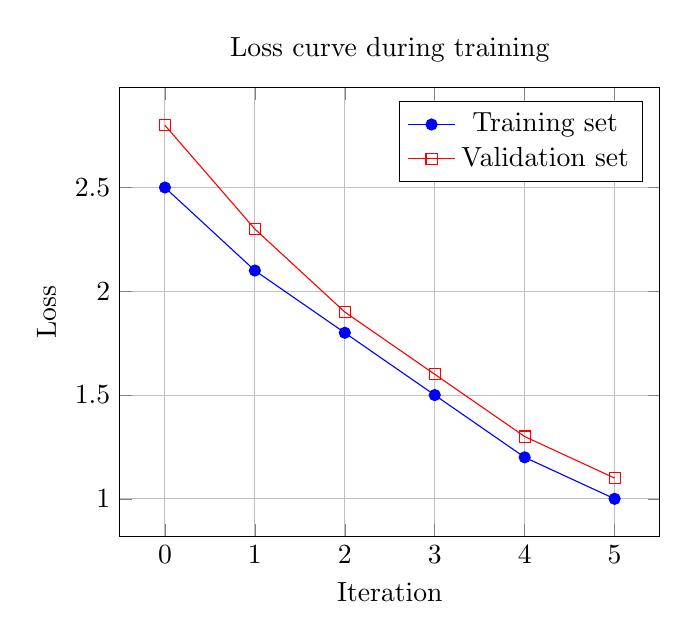
\begin{tikzpicture}
        \begin{axis}[
            xlabel={Iteration},
            ylabel={Loss},
            title={Loss curve during training},
            legend pos=north east,
            grid=major
        ]
        \addplot[color=blue,mark=*] coordinates {
            (0,2.5)
            (1,2.1)
            (2,1.8)
            (3,1.5)
            (4,1.2)
            (5,1.0)
        };
        \addplot[color=red,mark=square] coordinates {
            (0,2.8)
            (1,2.3)
            (2,1.9)
            (3,1.6)
            (4,1.3)
            (5,1.1)
        };
        \legend{Training set, Validation set}
        \end{axis}
    \end{tikzpicture}
    \caption{Example figure: Loss curve during training}
    \label{fig:loss-curve}
\end{figure} 

\section{Tables}
\begin{table}[htbp]
    \centering
    \caption{Example table: Performance comparison of different algorithms}
    \label{tab:algorithm-comparison}
    \begin{tabular}{lccc}
        \toprule
        Algorithm & Accuracy (\%) & Training time (s) & Memory usage (MB) \\
        \midrule
        Random Forest & 95.2 & 120 & 256 \\
        SVM & 93.8 & 180 & 128 \\
        Neural Network & 96.5 & 300 & 512 \\
        \bottomrule
    \end{tabular}
\end{table}

\listnotes
\bibliography{ref.bib}

% \nocite{*}

\end{document}
